\section{Datasets}
\label{sec:db}

The annotated segmentation and saliency datasets, which are used by the researchers to test the alforithms are often made available to the object saliency detection and segmentation community.

\subsection{Saliency Datasets}
\subsubsection{MSRA}
The MSRA  Database form the Visual computing group of Microsoft  research \cite{msra_db} is a collection of two image sets. The first set consists of $20 000$ images labelled by three users, while the second set consists of $5000$ images labelled by nine users. The labellings are available as bounding boxes. Figure \ref{fig:msra} illustrates the dataset.
\begin{figure}[H]
\begin{center}
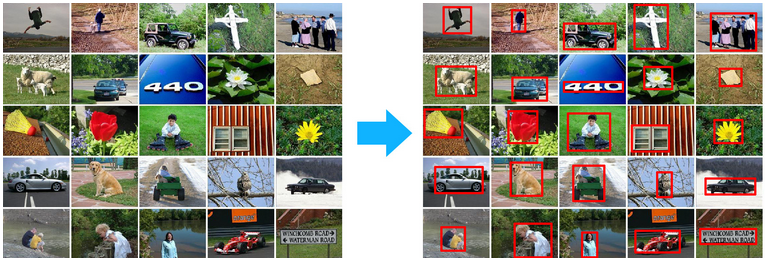
\includegraphics[width=0.95\textwidth]{fig/MSRA}
\end{center}
\caption{Examples of the MSRA dataset.}
\label{fig:msra}
\end{figure}
\subsubsection{MSRA10k}
This is an extension of the MSRA dataset, which  addresses the coarse-grained limitation of the MSRA labellings (bounding boxes). The MSRA10k (\cite{msra10k_db}) dataset consists of $10000$ randomly selected MSRA images for which a pixel-level saliency labelling is available. Figure \ref{fig:msra10k} illustrates the dataset. 
\begin{figure}[H]
\begin{center}
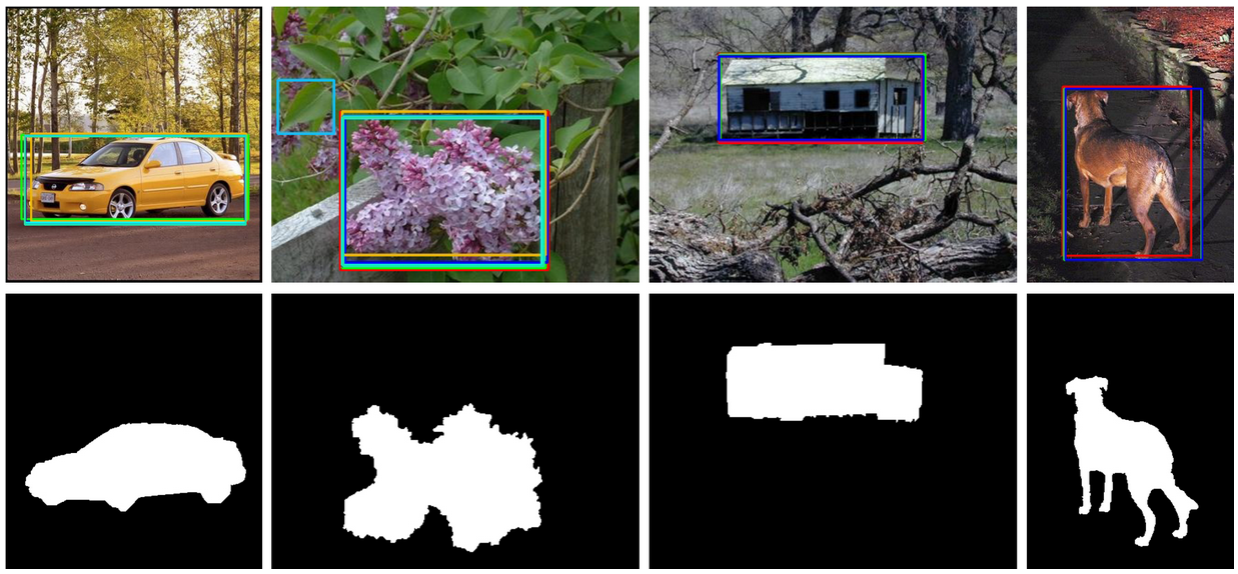
\includegraphics[width=0.95\textwidth]{fig/MSRA10k}
\end{center}
\caption{Examples of the MSRA 10k dataset. First row: original images with ground truth rectangles from MSRA dataset. Second row: Ground truth with pixel accuracy.}
\label{fig:msra10k}
\end{figure}
This dataset is used by in a very recent paper in IEEE Transactions on PAMI \cite{ChengPAMI2015} and \cite{chengPAMIUrl} (online resources with link to the software). 

\subsubsection{CSSD and ECSSD}
Although images from MSRA-1000 \cite{} have a large variety in their content, background structures are primarily simple and smooth. To represent the situations that natural images generally fall into, the Complex Scene Saliency Dataset (CSSD) \cite{} was proposed in \cite{}. The CSSD was extended to a larger dataset (ECSSD) with 1000 images, which includes many semantically meaningful but structurally complex images for evaluation. The images are acquired from the internet and 5 helpers were asked to produce the ground truth masks.The CSSD contains 200 and the ECSSD- 1000 images.
